Bár az elektronikusan közölt információk típusa (pl.: rekeszátmérő) nagyban ismert, hogy pontosan melyik elektronikus kontakt, pontosan milyen módon közli az információt ismeretlen. Így mind a Z-bajonett mind az F-bajonett elektronikus kommunikációja egy fekete dobozhoz hasonlítható. Ennek a rendszernek a feltárására célszerű megközelítés visszafejtéses módszereket alkalmazni. "A visszafejtés itt úgy van definiálva, mint egy bizonyos hardverhez készült specifikációk létrehozása valaki olyan által, aki nem tartozik az eredeti dizájnerek közé, elsősorban egy egyed vagy egyedek gyűjteményének analizálására vagy dimienziózására alapozva."\cite{Reverse_engineering}
\subsection{Elemek azonosítása}
Első lépésként a konkrét kontaktok által szállított információk jelentéseit kell meghatározni. Ehhez először rögzítenünk kell a kontaktok különböző bemenetére adott reakcióját. Így miközben egy objektív csatlakoztatva van, méréseket végzünk a kapcsolaton. Ezt az alábbi (\ref{fig:jelparosito_UML}) diagrammon látható rendszerrel valósíthatjuk meg. Itt a jel leírásánál fel kell tüntetni az áramerősséget és a feszültséget is, mivel mindkettő tartalmazhat szükséges információt.
\begin{figure}[H]
	\centering
	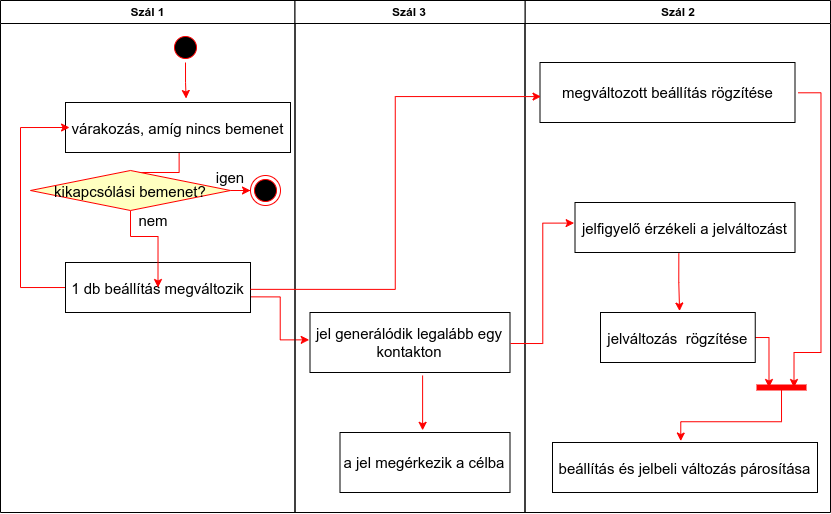
\includegraphics[width=1.0\linewidth]{img/Reverse_2.drawio.png}
	\caption{Nikon F (bal) és Nikon z (bal) objektívfoglalatok belső átmérője közti különbség}
	\label{fig:jelparosito_UML}
\end{figure}
Fontos a bemeneti és a kimeneti (jelek a kontaktokon) változásokat összepárósítani, mivel így a bemenetek alapján rendezve könnyebben meghatározható, hogy mely adatokért mely csatornák felelnek.
\subsubsection{Rögzítőberendezés}
A rögzítőberendezés nem feltétlenül képes minden kontaktot egyszerre felügyelni. Ilyenkor ugyan azokkal a beállításokkal meg kell ismételni a tesztet, addig amíg nem lesz tesztelve az összes kontakt az adott beállítással. Az objektív és a kameratest közé nem juthat be fény, ezért keskeny, alacsony feszültségű kábelekkel kell kivezetni a jeleket a csatlakozások belsejéből. Annak érdekében, hogy az objektív és a kamera ne sérüljön, célszerű egy olcsó makró toldógyűrűt beiktatni a kettő közé, és abba kialakítani a réseket, amiken keresztül a jelet ki lehet vinni a szerkezetből. Miután az eszköz elvégezte a méréseket a jelet továbbítani kell az objektívnek, hogy annak (ha van) válasza is rögzülhessen.
\begin{figure}[H]
	\centering
	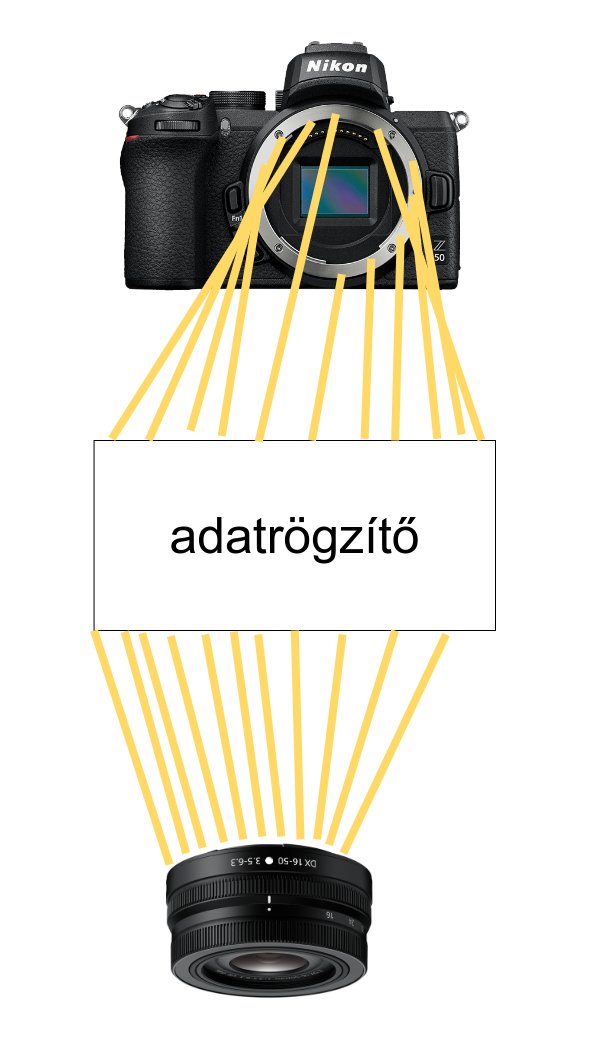
\includegraphics[width=0.5\linewidth]{img/arduino.drawio.png}
    \cite{Nikon_Z}\cite{Nikon_Z_16-50}
	\caption{Nikon Z interfész adatrögzítő}
	\label{fig:rogzito}
\end{figure}
\subsubsection{Mintavételezés}
A mintavételezésnek nem sokkal a beállítás megvéltozása elött kell kezdődnie, és a jel végeztável le kell állnia. Ezzel látványosan lehet szemléltetni az értékváltozást, és kinyerhetővé válik a jelváltozás szükséges sebessége, valamint a rögzítés megfelelően időzített leállításával elkerülhető a fölösleges feljegyzések generálása, ezzel csökkentve az adatfeldolgozással töltött időt.
\paragraph{Mintavételezési gyakoriság}
Mivel a jelet rögzítésnél az analízis érdekében analógként kezeljük (nem digitális 1 eseket és nullákat rögzítünk, hanem az elektromos jel fentebb említett tulajdonságainak értékeit rögzítjük), de digitálisan tároljuk, ezért meghatározott időközönként kell mintavételezést végeznünk. Ennek a gyakoriságát a e Nyquist-Shannon mintavételezési elmélet alapján határozzuk meg. "A Nyquist elmélet leírja, hogy hogyan lehet mintavételezni egy hullámból úgy, hogy ne vesszen el információ."\cite{por2019nyquist} Esszerint a mintavételezési gyakoriságnak a jel legnagyobb lehetséges frekvenciájának kétszeresének kell lennie (\ref{eq:Nyguist})\cite{por2019nyquist}.

\begin{align}
    f_{minta} \geq 2f_{max}
    \label{eq:Nyguist}
\end{align}	
\cite{por2019nyquist}

Ebből következik, hogy egy mintavételezési gyakoriság alapján meghatározható az a frekvencia, aminél kisebb, vagy azonos frekvenciájú jelek veszteség nélkül visszaállíthatóak (\ref{eq:Nyguist_freq}). Ez a frekvencia a Nyguist frekvencia.

\begin{align}
    f_{Nyguist} = \frac{1}{2}f_{max}
    \label{eq:Nyguist_freq}
\end{align}	
\cite{por2019nyquist}

A maximális frekvencia meghatározásához előbb a mintavételező maximális mintavételezési sebességét használva, interpolációval hozunk létre egy függvényt. Ezt elég minden kontakt esetén egyszer elvégezni, azonban több méréssel, és azok egyesítésével megbízhatóbb eredményt kapunk. Ilyenkor valószínűleg a szükségesnél nagyobb a mintavételezési frekvencia, ezért az interpolációt el lehet végezni. A függvény csúcsai közti idő felhasználásával határozzuk meg az $f_{max}$ frekvenciát. Ezt a (\ref{eq:csucsok}) képlettel kaphatjuk meg. A csúcsokat az g(idő) függvény deriválásával, a deriváltfüggvény zérushelyeinek meghatározásával, és a kapott helyek közül a pozitív függvényértéket felvevők kiválasztásával érdemes elvégezni.

\begin{align}
    f_{max} = \frac{1}{min^{n - 1}_{i = 1}(|t_{i} - t_{i + 1}|)}
    \label{eq:csucsok}
\end{align}	
\small Ahol $n$ a csúcsok száma és $t \in T$ a csúcs rögzítésének ideje.

Egy beállítással több mérést is kell végezni, így csökkentve az esélyét annak, hogy egy vagy több meghibásodásnak köszönhetően rossz konklúzióra jussunk. Az ideális tesztek számát a méréseket végző türelme, és a kapott értékek közti különbségek alapján lehet meghatározni.

\subsubsection{Adatok rendezése}
Hogy könnyebben értelmezhetőek legyenek az összegyűjtött adatok, azokat szűrni és egyesíteni kell.
\paragraph{Szűrés}
A szórást úgy végezzük el, hogy egy adott $t$ helynek $\epsilon$ környezetében vett adatoknak azt az intervallumát tartjuk meg, amely tartalmazza azoknak a 99\%-át. Ezt úgy tehetjük meg, hogy az adatokat növekvő sorrendbe rendezzük, kiszámoljuk a $i = \frac{AdatokDarabszáma}{2}*0.99$ lefelé kerekített képlettel kiszámoljuk a mediántól jobbra és balra lévő megtartandó adatok darabszámát. A rendezett, szükséges elemek indexei ilyenkor a $[n-i,n+i]$ intervallumon belülre esnek, ahol $n$ a medián indexe, és $i$ a fenti képlettel kiszámított környezet lefele ekerekítve. Amennyiben egy teszt tartalmaz ezen az intervallumon kívül eső adatot, akkor az érvénytelennek minősül, és az adatai nem használhatóak a következő lépésben.
\paragraph{Összefésülés}
Mivel az adatrögzítés a minden feljegyzés esetében, a beállításváltozáshoz képest ugyan akkor kezdődik, és ér véget, valamint a mintavételezési gyakoriság megegyezik, ezért az egy beállításhoz tartozó adatokat a mérés kezdése óta eltelt idő alapján csoportosíthatjuk. A fenti szűrés elvégzése után a több mintából egyet alakítunk ki úgy, hogy egy ilyen kategóriába tartozó adatoknak az átlagát vesszük, és az így keletkezett feljegyzésből állítjuk vissza az eredeti függvényt.
% ide le kellene írni, hogy hogyan kell visszaállítani.

\subsection{Jelek átalakítása}
Az adathalmaz kialakítása után értelmezni kell a kapott függvényeket, és azokból a bemenet alapján kinyerni az adatokat
\subsubsection{Analóg és digitális jelek elkülönítése}
Elektronikus úton két féle képpen lehetséges adatokat továbbítani. Az elektromos jel lehet digitális vagy analóg. A fenti adattranszformációk elvégzése után a függvényt vizualizálva könnyen megállapítható annak típusa következő módon. Amennyiben a függvény értéke két érték között váltakozik, azokat elérve ezeket az értékeket egy bizonyos ideig tarták, akkor ez egy négyzetfüggvény és digitális a jelre utal. Amennyiben a jel több értéket is felvesz, valamint hullámossága nagyobb, akkor a jel analóg.

\begin{figure}[H]
	\centering
	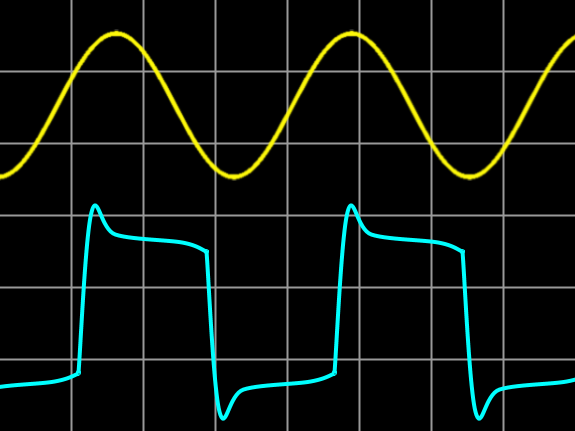
\includegraphics[width=0.5\linewidth]{img/oszcilloskóp.png}
    \cite{digital_vs_analog}
	\caption{Analóg (fent) és digitális (lent) az oszcilloskópon}
	\label{fig:oscilloszkop}
\end{figure}

\subsubsection{Analóg jelek transzformálása}
\paragraph{Analóg-Analóg kapcsolat}
Az ilyen típusú jelek pontos jelentését nehéz meghatározni. Ezért amennyiben az adott funkciót mind a Z és az F oldalon analóg jelek látják el, akkor az egyik oldalról kapott mintákon lineáris transzformációt végzünk úgy, hogy a másik oldal interfészének megfeleljen.
\paragraph{Analóg-Digitális kapcsolat}
Ebben az esetben kötelező értelmezni az analóg jelet. Ezt úgy lehet megtenni, hogy az ismert bemenettel asszociáljuk az adatgyűjtés során kapott analóg függvényt. Amennyiben a kapott analóg függvény eléggé hasonlít (a bemenet értékének, annak változásának, valamint a mintafügvény értékének, annak változásának, különbsége határártéken belül van), akkor kimeneti digitális jel az analóg jellel asszociált digitális jelet adja tovább. Amennyiben a jelet digitálisról kell analógra váltani, akkor a kimeneten a digitális jellel asszociált függvényt kell megjelentetni.

\subsubsection{Digitális jelek analizálása és transzformálása}
A digitális jelet elöször demodulárni kell (analógból digitálissá alakítani), miután megállapítottuk a moduláció módját az analóg forrás vizsgálatával. Amennyiben ezt támogatja a mikrokontroller bemenete, annyiban nem szükséges további szoftveres feldolgozást végezni az analóg jelen, máskülönben a demodulációt be kell iktatni a mikroprocesszoron futtatott szoftverbe. Ezt követően a bemenetből és az ipari szabványokból kiindulva dekódolni lehet az adatokat. Azonban ez a legtöbb esetben nem szükséges, mivel a cél a két interfész közti adatmegfeleltetés. Így elég egy hasítótábla segítségével kikeresni digitális jelbemenetnek megfelelő kimeneti adatláncot, és azt továbbküldeni. Amennyiben a két adatlánc közt matematikai összefüggés is leírható, akkor azt érdemes használni a transzformációra, a memóriaigény csökkentése, és a gyorsabb reakció érdekében.